\subsection{QA}
\begin{definition}
    \begin{enumerate}
        \item What does Fourier coefficients mean?
        \begin{itemize}
            \item It is the strength each complex exponential signal has. 
        \end{itemize}
    \end{enumerate}
\end{definition}

\subsection{FS Notation}
\begin{definition}
    If \( x(t) = \sum_{k \in \mathbb{Z}} c_k e^{j 2\pi \frac{k}{T} t} \), we write \( x \underset{T}{\overset{FS}{\longleftrightarrow}} c_k \) or \( x \overset{\text{FS}}{\longleftrightarrow} c_k \) if \( T \) is known.
\end{definition}

\begin{warning}
    We can find FS in terms of other FS we know. 
\end{warning}

\subsection{Properties of FS}
\begin{definition}
    \begin{enumerate}
        \item \textbf{Linearity:} If \( x \underset{T}{\overset{FS}{\longleftrightarrow}} a_k \) and \( y \underset{T}{\overset{FS}{\longleftrightarrow}} b_k \), then for all scalars \(\alpha_1, \alpha_2 \in \mathbb{C} \),
        \[
        \alpha_1 x + \alpha_2 y \underset{T}{\overset{FS}{\longleftrightarrow}} \alpha_1 a_k + \alpha_2 b_k
        \]
    
        \item \textbf{Time Reversal:} If \( x(t) \underset{T}{\overset{FS}{\longleftrightarrow}} c_k \), then \( \tilde{x}(t) = x(-t) \underset{T}{\overset{FS}{\longleftrightarrow}} c_{-k} \).
        \begin{itemize}
            \item $x_{\text{even}} = \frac{1}{2} \left( x + \tilde{x} \right) \underset{T}{\overset{\text{FS}}{\longleftrightarrow}} \frac{1}{2} \left( c_k + c_{-k} \right)$
            \item $x_{\text{odd}} = \frac{1}{2} \left( x - \tilde{x} \right) \underset{T}{\overset{\text{FS}}{\longleftrightarrow}} \frac{1}{2} \left( c_k - c_{-k} \right)$    
        \end{itemize}
    
        \item \textbf{Conjugation:} If \( x(t) \underset{T}{\overset{FS}{\longleftrightarrow}} c_k \), then \( x^*(t) \underset{T}{\overset{FS}{\longleftrightarrow}} c_{-k}^* \).
        \begin{itemize}
            \item $x^*(t) = (x(t))^*$
        \end{itemize}
        \begin{itemize}
            \item $\text{Re}(x) = \frac{1}{2} (x + x^*), \text{ so if } x \overset{\text{FS}}{\longleftrightarrow} c_k, \text{ then } \text{Re}(x) \longleftrightarrow \frac{1}{2} (c_k + c_{-k}^*)$
            \item $\text{Im}(x) = \frac{1}{2j} (x - x^*), \text{ so if } x \overset{\text{FS}}{\longleftrightarrow} c_k, \text{ then } \text{Im}(x) \longleftrightarrow \frac{1}{2j} (c_k - c_{-k}^*)$
            \begin{itemize}
                \item $c_k = c_{-k}^*$ if the signal is real, so it becomes $0$.
            \end{itemize}
        \end{itemize}
    
        \item \textbf{Time Scaling:} If \( x(t) \underset{T}{\overset{FS}{\longleftrightarrow}} c_k \), then \( x(at) \underset{T/a}{\overset{FS}{\longleftrightarrow}}c_k \) for \( a > 0 \), and \( x(at) \underset{T/(-a)}{\overset{FS}{\longleftrightarrow}} c_{-k} \) for \( a < 0 \).
        \begin{itemize}
            \item $-a$ is needed to be the period since $a<0$ so $-a>0$, and periods are defined for positive values. 
            \item \textbf{Note:} Period has changed, but the FS coefficients stay the same (i.e. spacing changes). This is why the notation is good to have. 
        \end{itemize}
    
        \item \textbf{Time Shifting:} If \( x(t) \underset{T}{\overset{FS}{\longleftrightarrow}} c_k \), then \( x(t - t_0) \underset{T}{\overset{FS}{\longleftrightarrow}}  e^{-j 2\pi \frac{k}{T} t_0} c_k \).
        \begin{itemize}
            \item The term \( e^{-j 2\pi \frac{k}{T} t_0} \) is a phase factor, so time-shifting alters the phase but not the magnitude of the FS coefficients.
        \end{itemize}
    
        \item \textbf{Multiplication:} If \( x(t) \underset{T}{\overset{FS}{\longleftrightarrow}} a_k \) and \( y(t) \underset{T}{\overset{FS}{\longleftrightarrow}} b_k \), then \( x(t) y(t) \underset{T}{\overset{FS}{\longleftrightarrow}} \sum_{n \in \mathbb{Z}} a_n b_{k-n} \).
        \begin{itemize}
            \item \textbf{Key:} Multiplication in time domain is convolution in frequency domain. Vice versa.
        \end{itemize}
        \item \textbf{Parseval's Relation:} If \( x \underset{T}{\overset{FS}{\longleftrightarrow}} c_k \), then

        \[
        \frac{1}{T} \int_{T} |x(t)|^2 \, dt = \sum_{k \in \mathbb{Z}} |c_k|^2
        \]
        \begin{itemize}
            \item \textbf{Note:} Sometimes LS is easier to compute and sometimes RS is easier to compute. 
            \item \textbf{English:} Total power of the signal in the time domain to the sum of the squared magnitudes of its Fourier series coefficients in the frequency domain.
        \end{itemize}

        \item \textbf{Modulation (frequency-shifting)} If $x(t) \underset{T}{\overset{\text{FS}}{\longleftrightarrow}} c_k$, then, for any \( m \in \mathbb{Z} \),
        
        \[
        x(t)e^{j\frac{2\pi m}{T}t} \underset{T}{\overset{\text{FS}}{\longleftrightarrow}} c_{k-m}
        \]        
        \item \textbf{Differentiation:} If $x(t) \underset{T}{\overset{\text{FS}}{\longleftrightarrow}} c_k$, then
        \[
        x'(t) \underset{T}{\overset{\text{FS}}{\longleftrightarrow}} j\frac{2\pi k}{T} c_k.
        \]
    \end{enumerate}     
\end{definition}

\begin{derivation}
    \begin{enumerate}
        \item \textbf{Linearity:} Follows from linearity of summation.
        \item \textbf{Time reversal:} 
        \[
        \tilde{x}(t) = x(-t) = \sum_{k \in \mathbb{Z}} c_k e^{j 2\pi \frac{k}{T} (-t)} = \sum_{k \in \mathbb{Z}} c_k e^{j 2\pi \frac{-k}{T} t}
        \]
        Let \( k' = -k \), so we get
        \[
        \tilde{x}(t) = \sum_{k' \in \mathbb{Z}} c_{-k'} e^{j 2\pi \frac{k'}{T} t}
        \]
        Therefore, \( \tilde{x}(t) \longleftrightarrow c_{-k} \).

        \item \textbf{Conjugation:} 
        \[
            x^*(t) = \left( \sum_{k \in \mathbb{Z}} c_k e^{j 2\pi \frac{k}{T} t} \right)^* = \sum_{k \in \mathbb{Z}} c_k^* e^{-j 2\pi \frac{k}{T} t}
            \]
            Let \( k' = -k \), then 
            \[
            x^*(t) = \sum_{k' \in \mathbb{Z}} c_{-k'}^* e^{j 2\pi \frac{k'}{T} t}
            \]
            Thus, \( x^*(t) \longleftrightarrow c_{-k}^* \).
        \item \textbf{Time scaling:}
        \textbf{Proof:} 
        \[
        x(at) = \sum_{k \in \mathbb{Z}} c_k e^{j 2\pi \frac{k}{T} (at)} = \sum_{k \in \mathbb{Z}} c_k e^{j 2\pi \frac{k}{T/a} t}, \quad \text{if } a > 0
        \]
        \vspace{1em}

        \begin{align*}
            x(at) &= \sum_{k \in \mathbb{Z}} c_k e^{j 2\pi \frac{-k}{T/(-a)} t}, \quad \text{if } a < 0 \\
            &\text{Let $k' = -k$} \\ 
            &= \sum_{k'\in \mathbb{Z}} c_{-k'} e^{j 2\pi \frac{k'}{T/(-a)} t}
        \end{align*}

        \item \textbf{Time shifting:}
        \[
        x(t - t_0) = \sum_{k \in \mathbb{Z}} c_k e^{j 2\pi \frac{k}{T} (t - t_0)} = \sum_{k \in \mathbb{Z}} c_k e^{-j 2\pi \frac{k}{T} t_0} e^{j 2\pi \frac{k}{T} t}
        \]

        \item \textbf{Multiplication:} For notational convenience, let \( \Omega(t) = e^{j 2\pi \frac{t}{T}} \), then for any integer \( \Omega^k(t) = e^{j 2\pi \frac{k}{T} t} \), \( k \in \mathbb{Z} \),
        \[
        x(t) = \sum_{n \in \mathbb{Z}} a_n \Omega^n(t), \quad y(t) = \sum_{m \in \mathbb{Z}} b_m \Omega^m(t)
        \]
        Therefore, 
        \[
        x(t) y(t) = \sum_{n \in \mathbb{Z}} a_n \Omega^n(t) \sum_{m \in \mathbb{Z}} b_m \Omega^m(t) = \sum_n \sum_m a_n b_m \Omega^{n+m}(t)
        \]
        Let \( k = n + m \) so $m=k-n$, then 
        \begin{equation*}
            x(t) y(t) = \sum_n \sum_k a_n b_{k-n} \Omega^k(t)
        \end{equation*}
        \[
        x(t) y(t) = \sum_k \left( \sum_n a_n b_{k-n} \right) \Omega^k(t)
        \]
        Thus, \( c_k = \sum_n a_n b_{k-n} \).

        \item \textbf{Parseval's Relation:} Use the multiplication property with \( y = x^* \).

        \[
        x \underset{T}{\overset{FS}{\longleftrightarrow}} c_k \quad \text{and} \quad x^* \underset{T}{\overset{FS}{\longleftrightarrow}} c_{-k}^*
        \]
        
        Then, 
        
        \[
        x x^* \underset{T}{\overset{FS}{\longleftrightarrow}} a_k =  \sum_{n \in \mathbb{Z}} c_n c_{-(k-n)}^* = \sum_{n \in \mathbb{Z}} c_n c_{n-k}^*
        \]

        If \( k = 0 \),

        \[
        a_0 = \sum_{n \in \mathbb{Z}} |c_n|^2 = \frac{1}{T} \int_{T} |x(t)|^2 \, dt
        \]
        \begin{itemize}
            \item \textbf{Note:} RS comes from the analysis equation of $x x^*$.
        \end{itemize}

        \item \textbf{Modulation:}  \[
            x(t)e^{j\frac{2\pi m}{T}t} \underset{T}{\overset{\text{FS}}{\longleftrightarrow}} a_k
            \]
            
            Then, by the analysis equation:
            
            \[
            a_k = \frac{1}{T} \int_T x(t) e^{j\frac{2\pi m}{T}t} e^{-j\frac{2\pi k}{T}t} dt
            \]
            
            \[
            = \frac{1}{T} \int_T x(t) e^{-j\frac{2\pi (k - m)}{T}t} dt = c_{k-m}
            \]
        
        \item \textbf{Differentiation:} We know that by the synthesis equation:
        \[
        x'(t) = \frac{d}{dt} \sum_{k \in \mathbb{Z}} c_k e^{j\frac{2\pi k}{T}t}
        \]
        
        Taking the derivative,
        \[
        x'(t) = \sum_{k \in \mathbb{Z}} c_k \frac{d}{dt} \left( e^{j\frac{2\pi k}{T}t} \right)
        \]
        
        \[
        = \sum_{k \in \mathbb{Z}} c_k \cdot j\frac{2\pi k}{T} e^{j\frac{2\pi k}{T}t}
        \]
        
        Thus,
        \[
        x'(t) \underset{T}{\overset{\text{FS}}{\longleftrightarrow}} j\frac{2\pi k}{T} c_k
        \]
    \end{enumerate}
\end{derivation}

\begin{warning}
    The substitution of $-k=k'$ is made so the basis vectors remain intact, since for all of these $x(t)$, the basis set must always be $x(t) = \sum_{k \in \mathbb{Z}} c_k e^{j 2\pi \frac{k}{T} t}$.
\end{warning}

\subsubsection{Consequences of even,odd,imaginary,real}

\begin{intuition}
    \begin{enumerate}
        \item If $x(t)$ is even: 
        \begin{equation*}
            c_k = c_{-k}
        \end{equation*}
        \begin{itemize}
            \item Calculate only half of the FS coefficients and infer the others with conjugate symmetry.
        \end{itemize}
        \item If $x(t)$ is odd:
        \begin{equation*}
            c_k = - c_{-k}
        \end{equation*}
        \item If $x(t)$ is real:
        \begin{equation*}
            c_k = c_{-k}^*
        \end{equation*}
        \item If $x(t)$ is imaginary:
        \begin{equation*}
            c_k = - c_{-k}^*
        \end{equation*}    
        \item If \( x(t) \) is even and real: 
        \begin{equation*}
            c_k = c_{-k}
        \end{equation*}
        \begin{itemize}
            \item Only cosine contributes.
        \end{itemize}
        
        \item If \( x(t) \) is even and imaginary: 
        \begin{equation*}
            c_k = -c_{-k}
        \end{equation*}
    
        \item If \( x(t) \) is odd and real: 
        \begin{equation*}
            c_k = -c_{-k}
        \end{equation*}
        \begin{itemize}
            \item Only sine contributes.
        \end{itemize}
    
        \item If \( x(t) \) is odd and imaginary: 
        \begin{equation*}
            c_k = - c_{-k}
        \end{equation*}

        \item Decompose any signal \(x(t)\) into its \textbf{even} and \textbf{odd} parts using:
            \[
            x_{\text{even}} \overset{\text{FS}}{\longleftrightarrow} \frac{1}{2} (c_k + c_{-k}), \quad x_{\text{odd}} \overset{\text{FS}}{\longleftrightarrow} \frac{1}{2} (c_k - c_{-k})
            \]

        \item  If \(x(t)\) is complex, decompose it into its \textbf{real} and \textbf{imaginary} parts:
        \[
        \text{Re}(x) \overset{\text{FS}}{\longleftrightarrow} \frac{1}{2}(c_k + c_{-k}^*), \quad \text{Im}(x) \overset{\text{FS}}{\longleftrightarrow} \frac{1}{2j}(c_k - c_{-k}^*)
        \]

        \begin{itemize}
            \item To figure out these relationships, just look at the converse. i.e. if x is even, then look at odd case because it has to be 0. Vice versa for real, imaginary, and odd.
            \item DOUBLE CHECK THE COMBINATION ONES.
        \end{itemize}

    \end{enumerate}
    
\end{intuition}

\subsubsection{Intuition on modulation:}
\begin{intuition}
    \customFigure[0.75]{00_Images/MOD.png}{Modulation with the complex exponential results in a shift by $m$}
    \customFigure[0.75]{00_Images/MOD1.png}{Cosine}
    \begin{itemize}
        \item Modulation with the cosine results in two different frequency packs shifted by $m$. The negative freqencies represent the phasor going CW. The positive frequencies represent the phasor going CCW, which cancel out to be only on the real part.
    \end{itemize}
    \customFigure[0.75]{00_Images/MOD2.png}{Product}
    \begin{itemize}
        \item The product of $x(t)$ with a high frequency cosine results in an envelope bounded by $x(t)$ since cosine is bounded by $1,-1$, $x(t)$ controls the amplitude (i.e. envelope), then the product is inside the envelope, which is at high frequency.
    \end{itemize}
\end{intuition}

\subsection{Example using properties}
\begin{example}
    Derive the square wave Fourier conefficients from the Impulse train to showcase how different properties are used (i.e. shifting, differentiation,linearity).
    \begin{enumerate}

        \item \textbf{The impulse train is given by:}
        \[
        p_T(t) = \sum_{k \in \mathbb{Z}} \delta(t - kT)
        \]

        \begin{center}
            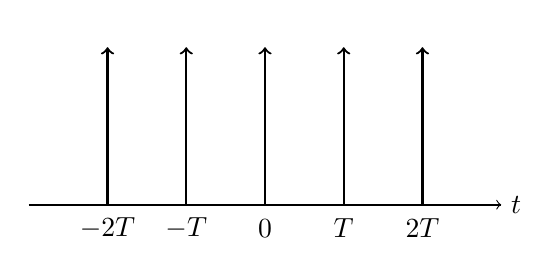
\begin{tikzpicture}
                % Draw the x-axis
                \draw[->] (-3,0) -- (3,0) node[right] {$t$};
                
                % Draw impulses at -2T, -T, 0, T, 2T
                \draw[->, thick] (-2,0) -- (-2,2) node[above] {};
                \draw[->, thick] (-1,0) -- (-1,2) node[above] {};
                \draw[->, thick] (0,0) -- (0,2) node[above] {};
                \draw[->, thick] (1,0) -- (1,2) node[above] {};
                \draw[->, thick] (2,0) -- (2,2) node[above] {};
                
                % Label the points -2T, -T, 0, T, 2T
                \node at (-2,-0.3) {$-2T$};
                \node at (-1,-0.3) {$-T$};
                \node at (0,-0.3) {$0$};
                \node at (1,-0.3) {$T$};
                \node at (2,-0.3) {$2T$};
                
                % Draw the baseline
                \draw[thick] (-3,0) -- (3,0);
                
            \end{tikzpicture}
        \end{center}
        
        \item \textbf{Fourier Series Coefficient of the Impulse Train:}
        \[
        p_T(t) \underset{T}{\overset{\text{FS}}{\longleftrightarrow}} a_k = \frac{1}{T} \int_{-T/2}^{T/2} \delta(t) e^{-j\frac{2\pi k}{T}t} dt
        \]
    
        \item \textbf{For \( t = 0 \) (i.e. when the impulse occurs within the interval):}
        \[
        a_k = \frac{1}{T} \int_{-T/2}^{T/2} e^0 dt = \frac{1}{T}
        \]

    
        \item \textbf{For \( g(t) \), Fourier series coefficients are unknown:}
        \[
        g(t) \underset{T}{\overset{\text{FS}}{\longleftrightarrow}} c_k = ?
        \]
        \begin{center}
            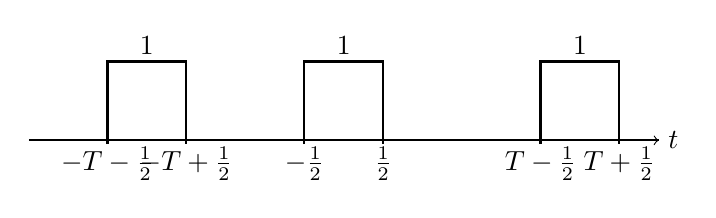
\begin{tikzpicture}
                % Draw the x-axis
                \draw[->] (-4,0) -- (4,0) node[right] {$t$};
            
                % Draw the square wave at -T-1/2 to -T+1/2
                \draw[thick] (-3,-0.05) -- (-3,1) -- (-2,1) -- (-2,-0.05);
                
                % Draw the square wave at -1/2 to 1/2
                \draw[thick] (-0.5,-0.05) -- (-0.5,1) -- (0.5,1) -- (0.5,-0.05);
                
                % Draw the square wave at T-1/2 to T+1/2
                \draw[thick] (2.5,-0.05) -- (2.5,1) -- (3.5,1) -- (3.5,-0.05);
                
                % Label the points -1/2, 1/2, T, -T-1/2, -T+1/2
                \node at (-3,-0.3) {$-T - \frac{1}{2}$};
                \node at (-2,-0.3) {$-T + \frac{1}{2}$};
                \node at (-0.5,-0.3) {$-\frac{1}{2}$};
                \node at (0.5,-0.3) {$\frac{1}{2}$};
                \node at (2.5,-0.3) {$T - \frac{1}{2}$};
                \node at (3.5,-0.3) {$T + \frac{1}{2}$};
            
                % Draw the baseline
                \draw[thick] (-4,0) -- (4,0);
                
                % Label the amplitude
                \node at (0,1.2) {1};
                \node at (3,1.2) {1};
                \node at (-2.5,1.2) {1};
            
            \end{tikzpicture}
        \end{center}
    
        \item \textbf{Derivation of \( q(t) \):}
        \begin{align*}
        q(t) &= \frac{d}{dt} g(t) = p_T \left( t + \frac{1}{2} \right) - p_T \left( t - \frac{1}{2} \right)
        \end{align*}

        \begin{center}
            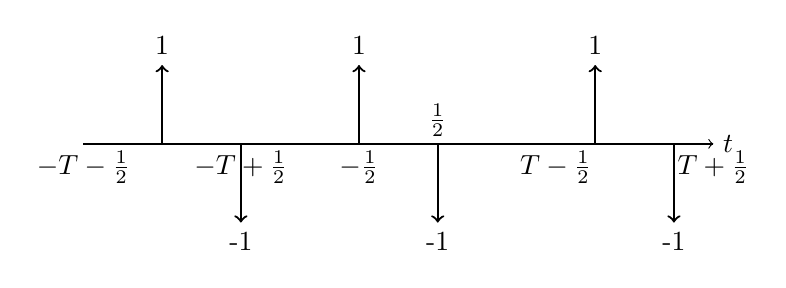
\begin{tikzpicture}
                % Draw the x-axis
                \draw[->] (-4,0) -- (4,0) node[right] {$t$};
            
                % Draw the impulses at -T-1/2 to -T+1/2
                \draw[->, thick] (-3,0) -- (-3,1) node[above] {1};
                \draw[->, thick] (-2,0) -- (-2,-1) node[below] {-1};
                
                % Draw the impulses at -1/2 to 1/2
                \draw[->, thick] (-0.5,0) -- (-0.5,1) node[above] {1};
                \draw[->, thick] (0.5,0) -- (0.5,-1) node[below] {-1};
                
                % Draw the impulses at T-1/2 to T+1/2
                \draw[->, thick] (2.5,0) -- (2.5,1) node[above] {1};
                \draw[->, thick] (3.5,0) -- (3.5,-1) node[below] {-1};
                
                % Label the points -1/2, 1/2, T, T+1/2, -T-1/2
                \node at (-4,-0.3) {$-T - \frac{1}{2}$};
                \node at (-2,-0.3) {$-T + \frac{1}{2}$};
                \node at (-0.5,-0.3) {$-\frac{1}{2}$};
                \node at (0.5,0.3) {$\frac{1}{2}$};
                \node at (2,-0.3) {$T - \frac{1}{2}$};
                \node at (4,-0.3) {$T + \frac{1}{2}$};
            
                % Draw the baseline
                \draw[thick] (-4,0) -- (4,0);
            
            \end{tikzpicture}
        \end{center}
        
        \item \textbf{For \( p_T \left( t - \frac{1}{2} \right) \):}
        \begin{align*}
        p_T \left( t - \frac{1}{2} \right) &\underset{T}{\overset{\text{FS}}{\longleftrightarrow}} \frac{1}{T} e^{-j\frac{2\pi k}{T} \cdot \frac{1}{2}} = \frac{1}{T} e^{j\frac{-\pi k}{T}}
        \end{align*}
    
        \item \textbf{For \( p_T \left( t + \frac{1}{2} \right) \):}
        \begin{align*}
        p_T \left( t + \frac{1}{2} \right) &\underset{T}{\overset{\text{FS}}{\longleftrightarrow}} \frac{1}{T} e^{j\frac{2\pi k}{T} \cdot \frac{1}{2}} = \frac{1}{T} e^{j\frac{\pi k}{T}}
        \end{align*}
        \begin{itemize}
            \item $p_T \left( t + \frac{1}{2} \right) = p_T \left( t - \left(- \frac{1}{2}\right) \right)$.
        \end{itemize}
    
        \item \textbf{For \( q(t) \):}
        \begin{align*}
        q(t) &\underset{T}{\overset{\text{FS}}{\longleftrightarrow}} \frac{1}{T} \left( e^{j \frac{\pi k}{T}} - e^{-j \frac{\pi k}{T}} \right) = \frac{2j}{T} \sin \left( \frac{k \pi}{T} \right) = b_k
        \end{align*}
    
        \item \textbf{Relating \( q(t) \) and \( g(t) \):}
        \begin{align*}
        g(t) &=  \underset{T}{\overset{\text{FS}}{\longleftrightarrow}} c_k \\
        q(t) &= g'(t) \underset{T}{\overset{\text{FS}}{\longleftrightarrow}} b_k = j \frac{2 \pi k}{T} c_k
        \end{align*}
    
        \item \textbf{For \( k \neq 0 \):}
        \begin{align*}
        c_k &= \frac{b_k}{j \frac{2 \pi k}{T}} = \frac{\frac{2j}{T} \sin \left( \frac{k \pi}{T} \right)}{j \frac{2 \pi k}{T}} = \frac{1}{T} \text{sinc} \left( \frac{k}{T} \right)
        \end{align*}
    
        \item \textbf{For \( k = 0 \):}
        \begin{align*}
        c_0 &= \frac{1}{T} \int_T g(t) e^{-j \frac{2 \pi k t}{T}} dt = \frac{1}{T}
        \end{align*}
    
        \item \textbf{Thus, for \( g(t) \):}
        \[
        g(t) \underset{T}{\overset{\text{FS}}{\longleftrightarrow}} c_k = \frac{1}{T} \text{sinc} \left( \frac{k}{T} \right)
        \]
    
    \end{enumerate}
\end{example}